\begin{comment}

To cover:

- Description of the physics that cause the variable soil moisture
- Modeling this
  - Correy & Brooks
  - van Genuchten

- Description of van Genuchten


\end{comment}
% TODO: How do I cite here when I basically use the same source for everything?

\subsection{The Importance Of Soil Moisture Content}\label{sec:van_genuchten}

The portion of soil between groundwater and ground surface is variably saturated with water and is called the vadose zone.
Under environmental conditions, TCE and many other contaminants are miscible in water, and will be partitioned between water and vapor phases, which has profound effects on the total contaminant transport in the vadose zone.
The rates of diffusion in liquids and gases usually differ by orders of magnitudes.
Likewise, advective transport in the two phases occurs at vastly different rates, and as such it is important to account for the effects of soil moisture content on transport of contaminant.\par

Water filling of soil pores from the groundwater surface is driven by a negative pressure gradient induced by surface tension, called capillary potential and is here represented by $\psi$.
This capillary potential is a function of the soil moisture content, and becomes increasingly negative as the water content decreases, and is zero when the soil matrix is saturated with water.
The capillary potential varies with the hydraulic properties of specific soil types.\par

In addition to the capillary potential, soil moisture content is driven by a gravitational potential acting on water in the soil.
The total soil moisture potential $\phi$, is the sum of the capillary and gravitational potentials, here expressed as a pressure head.
\begin{equation}
  \phi = \frac{\psi(\theta_w)}{\rho g} + h_\mathrm{g} = h + h_\mathrm{g}
\end{equation}
where $\phi$ [\si{\metre}] is the total soil moisture potential;
$\psi$ [\si{\pascal}] is the capillary potential;
$h$ [\si{\metre}] is the capillary potential expressed as a pressure head above the groundwater/soil interface;
$\theta_w$ is the volumetric moisture content by volume soil, i.e. dimensionless;
$\rho$ [\si{\kilo\gram\per\metre\cubed}] is the density of water;
$g$ [\si{\metre\per\second\squared}] is the acceleration due to gravity;
and $h_\mathrm{g}$ [\si{\metre}] is the gravitational potential above a reference plane.\par

In the VI scenario considered here, we assume that there is no gravitational potential and the soil moisture content is at steady-state.
Thus, the soil moisture content is entirely determined by the capillary potential $h$.\par

There are two common methods for modeling the capillary potential, one developed by \citeauthor{brooks_properties_1966}\cite{brooks_properties_1966} in 1966, and another by \citeauthor{van_genuchten_closed-form_1980}\cite{van_genuchten_closed-form_1980} in 1980.
Both of these are semi-empirical approaches and relies on experimentally determined parameters for a specific soil type to be used.
In this work, we only use van Genuchten's method, simply because parameters for a wide variety of soils have been made available by the EPA (Table \ref{tbl:soils}).\par

\subsubsection{van Genuchten's Soil-Water Retention Model}

% TODO: Make sure the sign or absolute |h| should be here or not.
The relationship between capillary pressure and moisture content is called \textit{soil moisture retention}, and is what van Genuchten's method describes.
Specifically, his method models the water saturation of the soil and is given by \eqref{eq:van_genuchten_saturation}.
\begin{equation}\label{eq:van_genuchten_saturation}
  \mathrm{Se} =
    \begin{cases}
      \frac{1}{(1 + (\alpha |h|)^n)^m} & h < 0 \\
    1 & h \geq 0
    \end{cases}
\end{equation}
here $\mathrm{Se}$ is the saturation, which ranges from 0 to 1, where 1 is fully saturated with water;
$\alpha$, $m$, and $n=\frac{1}{1-m}$ are the empirically determined van Genuchten parameters given in Table \ref{tbl:soils};
and $h$ [\si{\metre}] is the capillary pressure head, which in this case is the elevation above the groundwater/soil interface.\par

It is important to note that $\mathrm{Se} = 0$ does not mean that there is no moisture in the soil; soils retain a small amount of water in the matrix - residual moisture content (which is soil specific).
Thus, the soil moisture content is given by \eqref{eq:van_genuchten_soil_moisture}
\begin{equation}\label{eq:van_genuchten_soil_moisture}
  \theta_w =
    \begin{cases}
      \theta_r + \mathrm{Se}(\theta_t - \theta_r) & h < 0 \\
      \theta_t & h \geq 0
    \end{cases}
\end{equation}
where $\theta_w$ is the volumetric soil moisture content;
$\theta_t$ is the soil porosity;
and $\theta_r$ is the residual moisture content.\par

By extension, the soil gas or air content is given by
\begin{equation}\label{eq:gas_porosity}
  \theta_g = \theta_t - \theta_w
\end{equation}
An example of the soil saturation and moisture content as a function of height above groundwater is shown in Figure \ref{fig:retention_curve}.
Note the steep decline in moisture content near the groundwater interface - that is the capillary zone and we will see that this zone presents a significant barrier to contaminant transport from the groundwater in section \ref{sec:transport}.\par

\begin{figure}
  \centering
  \begin{subfigure}[t]{0.49\textwidth}
    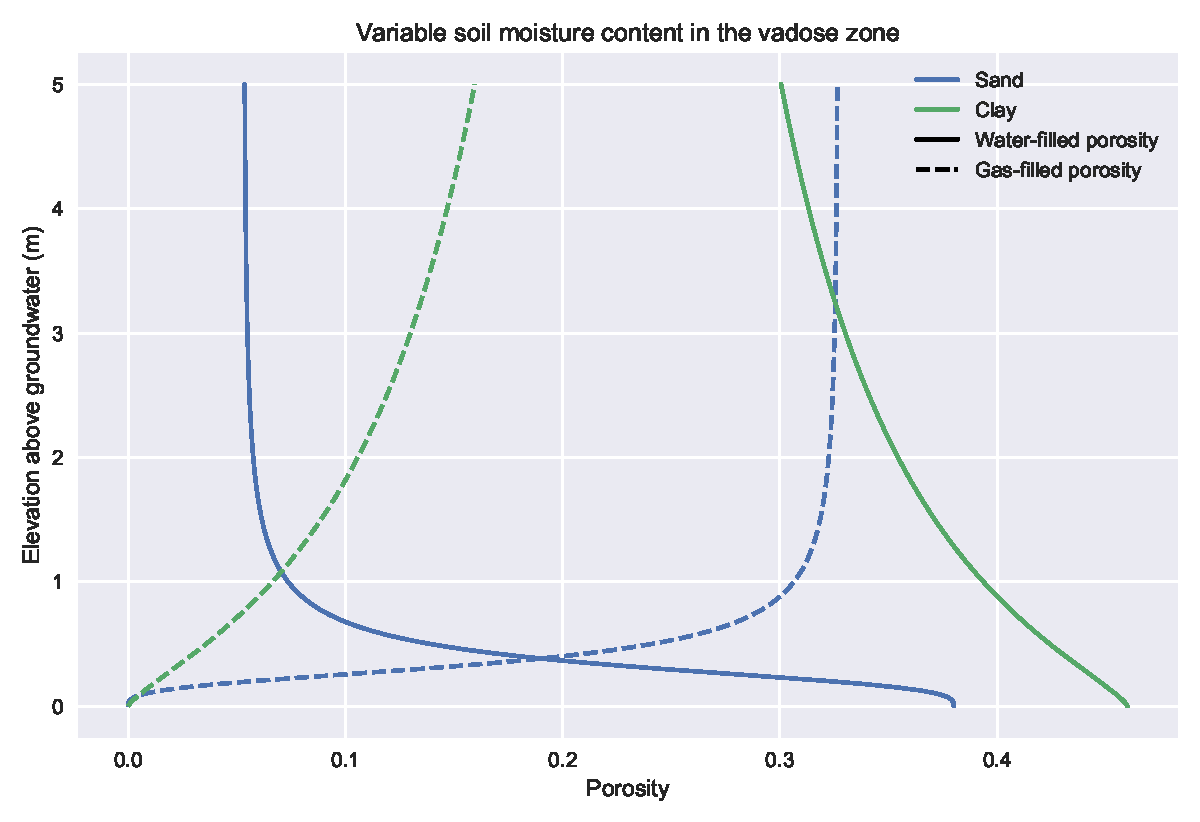
\includegraphics[width=\textwidth]{van_genuchten.pdf}
    \caption{Example of a soil moisture retention curve as a function of pressure head above the groundwater/soil interface.}
    \label{fig:retention_curve}
  \end{subfigure}
  \begin{subfigure}[t]{0.49\textwidth}
    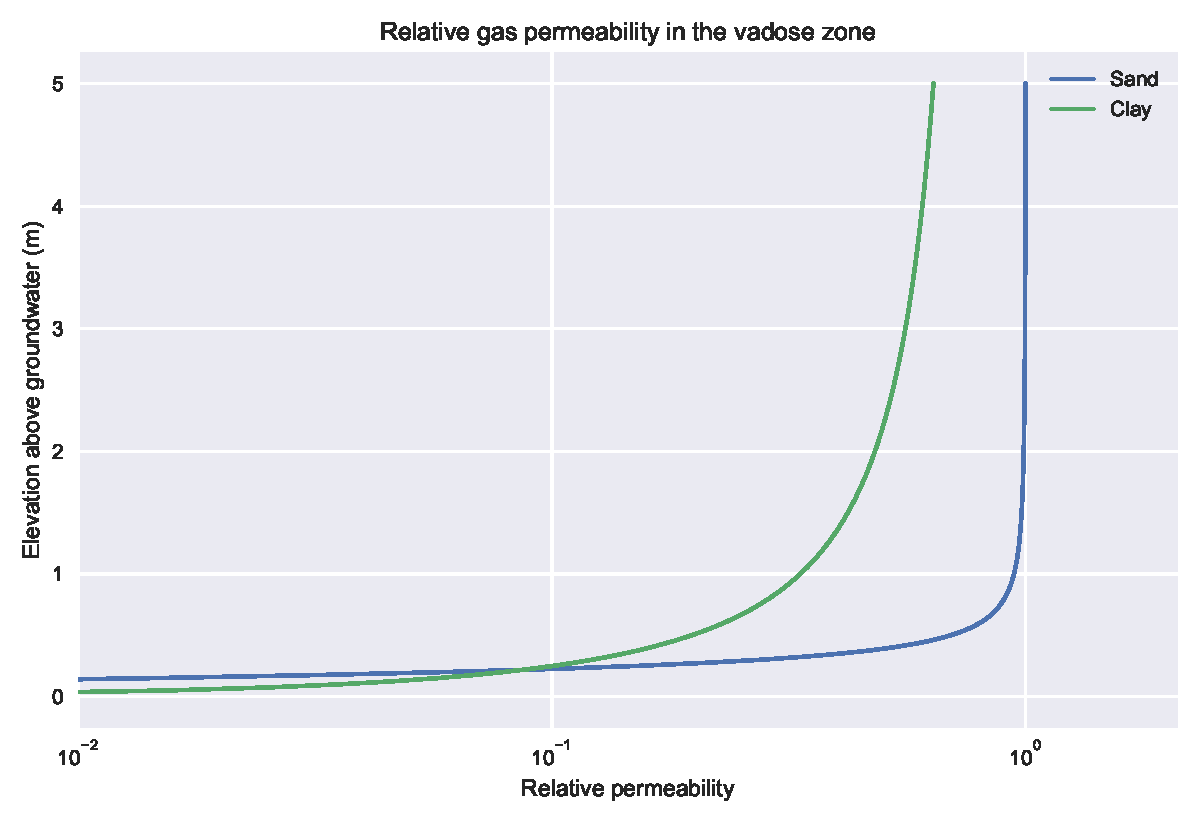
\includegraphics[width=\textwidth]{relative_permeability.pdf}
    \caption{Relative gas and water permeability in the vadose zone or above the groundwater interface.}
    \label{fig:relative_permeability}
  \end{subfigure}
\end{figure}

The presence of water in the soil matrix has profound implications for transport as the pore space may be restricted to only one phase.
For instance, in the capillary zone, contaminant transport is mostly limited by the water phase, while gas phase transport is extremely limited because air-filled porosity is limited and largely isolated.
The opposite is true near the ground surface, where most of the pore space is filled with air.\par

Soil already limits transport, i.e. it is harder to pump water through a soil columns than a pipe of the same size.
This extra phase-specific transport inhibition is modeled by a \textit{relative permability} and is given by \eqref{eq:van_genuchten_relative_permeability}.
\begin{equation}\label{eq:van_genuchten_relative_permeability}
  k_r =
    \begin{cases}
      \mathrm{Se}^l \big[ 1 - \big( 1 - \mathrm{Se}^\frac{1}{m} \big) \big]^2 & h < 0 \\
      0 & h \geq 0
    \end{cases}
\end{equation}
here $k_r$ is the relative permeability for water; % TODO: Make sure that is right
and $l = 0.5$ is another van Genuchten parameter.\par % TODO: How do I motivate this?

The relative permeability varies from 0 to 1, where 0 indicates that the soil matrix is completely impermeable to the fluid, while a value of 1 means that there is no additional permeability cost.
Since $k_r$ here is in relation to water, the relative permeability in relation to the vapor-phase is given by $1 - k_r$.
Figure \ref{fig:relative_permeability} shows how the relative gas permeability varies in the vadose zone.\par

\subsection{Including Gravitational Potential}
% TODO finish this
In this considered scenario, we assume that there is no gravitational potential acting on the water in the soil; there is no water flow occurring in the soil.
If this assumption cannot be made, e.g. the groundwater level is fluctuating over time, then the soil moisture content must be determined by Richard's equation.

If the assumption that there is no gravitational potential cannot be made, then the full soil moisture potential $\phi$ needs to be determined.
This is achieved by solving Richard's equation.\par % TODO: Write about Richard's equation and reference it?

\begin{comment}
% TODO: Move this to where Richard's equation is described.
\begin{equation}\label{eq:van_genuchten_moisture_capacity}
  C_m =
    \begin{cases}
      \frac{\alpha m}{1-m}(\theta_s - \theta_r)\mathrm{Se}^{\frac{1}{m}}\big( 1 - \mathrm{Se}^{\frac{1}{m}} \big)^m & h < 0 \\
    0 & h \geq 0
    \end{cases} \\
\end{equation}
\end{comment}
